\chapter{Implementation of RTM} % (fold)

\label{sec:Implementation of FPGA}

The paradigm of coding in FPGA is different from that in general purpose
coding, such as C/C++. To be more precise, it is called describing rather
than coding. Imaging the data flowing through the chip, and you are
designing a filter in the chip that can make some operation on the data.

When you are designing the kernel with Java, the code that you write
doesn't have a directly impact to the configuration of FPGA. Instead, the
Maxcompiler will endeavor to figure out the meaning of the code, or the
logic of the code, and the compiler will then generate the hardware
description language for the chip. So, you can also be convinced that you
are communicating with the compiler, rather than the chip directly.

\section{Streaming in FPGA} % (fold)
\label{sub:Streaming in FPGA}

To have the whole array processed, the host program (c/c+) usually use the
for loop to iterate through each element: make action to the element, and
then iterate next one. Such a loop is replaced by the streaming concept of
FPGA. So you don't need to write loop in the FPGA kernel design. You only
need to design the filter filtering each element.

Here I present a basic example of kernel designing to illustrate the
concept of FPGA designing, or paradigm. If we want to make a linear
transformation (equation (\ref{eq:fx})
to a vector, that is, to each element to the vector, a single for loop will
intuitive come to our mind.

\begin{equation}
  f(x) = 2x + 3
  \label{eq:fx}
\end{equation}

The pseudo code is shown in Listing (\ref{lst:fx}), which is unnecessary to
to explain. In this example, each element is applied to the function
(\ref{eq:fx}). The first element is processed first, then the second one,
and next and next. It is controlled with the help of the \emph{for} loop.
In FPGA kernel designing, data are streamed to the kernel, one by one. So
we don't have to write the for loop explicitly, instead, we are only
concentrate on the filter (in this example, the transformation).

\begin{figure}
  \centering
  \lstinputlisting[
    caption={Pseudo code of the transformation \( f(x) = 2x + 3 \) to a
    vector},
    label={lst:fx}
  ]{code/fx.c}
\end{figure}

Thus the first thing to do while designing the FPGA kernel is to specify
the input stream where the data from one by one and output stream where the
data goes one by one. We can achieve it using the given API. The core of
the kernel is designing how each data should processed, in this example,
that is the simple transformation. The code snippet is shown in listing
(\ref{lst:fx_kernel}).

\begin{figure}
  \centering
  \lstinputlisting[
    caption={Code snippet of the FPGA kernel of transformation to a
    vector},
    label={lst:fx_kernel},
    language={java}
  ]{code/fx_kernel.java}
\end{figure}

As you can see from the code snippet of the kernel, which is written in
Java, that there is no loop through out the kernel. The only one controlled
instruction is the transformation listed in line 9. The concept
\emph{streaming} is really import in FPGA designing because we are
designing a circuit, in particular, we are connecting the wires of the
circuit. In this example, we need an electrical element to perform the
multiplication and an element to perform the addition. These requirement
are issued by only one line of code (line 9). Then the Maxcompiler will
generate the target code, the hardware description code. So, in my
opinion, we are talking to the Maxcompiler and the Maxcompiler will make
a translation for us. Figure (\ref{fig:fx}) shows a graphical representation
of this kernel.

\begin{figure}
  \centering
  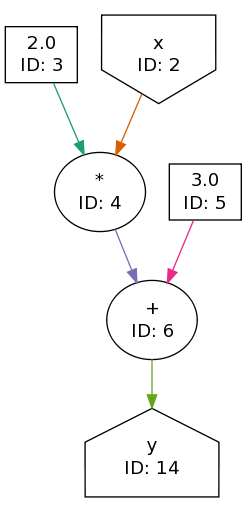
\includegraphics[scale=0.5]{img/SimpleKernel_original.png}
  \caption{Graph for a simple kernel}
  \label{fig:fx}
\end{figure}

In most cases, designing a kernel is not as simple as the previous example,
especially when the data to the stream is not independent. Most of time,
the FPGA designer are analyzing the algorithm and trying to cut the
relationship between the data. The more independent of the data, the easier
to design the kernel.

% section Streaming in FPGA (end)

\section{1D stencil design in FPGA} % (fold)
\label{sub:1D stencil design in FPGA}



The performance of the stencil operation is the key to the performance to
the whole application, as the RTM algorithm keeps calculating the stencil
operation. To have a better understanding of FPGA designing, we consider
the 1D-stencil design in FPGA rather diving into the 3D-stencil.

Apart from the previous example, which is only a simple transformation to
one element of the vector, where each element is independent, the neighbors
of the element is required to perform the stencil action. However, the
element is streamed to the kernel for each cycle. So, the point is, how to
attract the data that is in the future or in the past.

Stream offsetting allows us to access data elements within a stream
relative to the current location\cite{maxcompiler_tutorial}. The distance
from the largest to the smallest offset forms the window of data that must
be held on the FPGA on-chip memory. What's more, the core concept of stream
computing is operating on windows into data streams. Not only does the data
window is held in on-chip memory on the FPGA, and the data items are held
on-chip for exactly the amount of time required. This means good use of
on-chip memory use, since data is held for only so long as it is needed
rather than reload. And it also means good use of on-chip memory capacity,
since the data is held for only so long as it is needed.

\begin{figure}
  \centering
  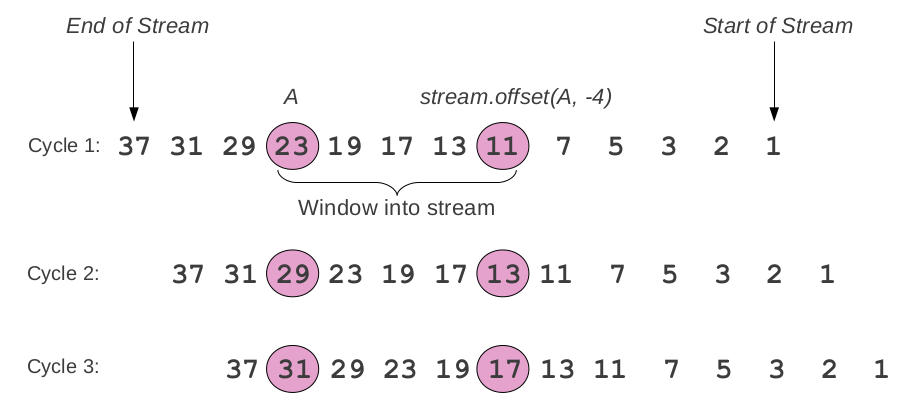
\includegraphics[scale=0.4]{img/window.png}
  \caption{Stream offsets from a window into a data stream}
  \label{fig:stream_window}
\end{figure}

Figure (\ref{fig:stream_window}) show a data stream A over three cycles.
The first element of the stream is 1, and the last element of the stream is
37. The current location will move from one location to next of each cycle.
Now, the current location (head of the stream) is A, which has the value
23. A kernel program accessing the head of the stream and also a data item
four elements into the past (with a value of 11 in cycle 1) create a window
of size five into stream A. Each cycle, the data in the stream moves
through the window.

\begin{figure}
  \centering
  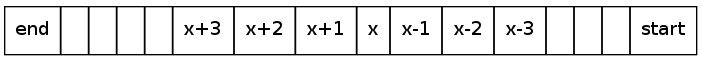
\includegraphics[scale=0.5]{img/array.png}
  \caption{Points for 1D array for stencil operation}
  \label{fig:array}
\end{figure}

\begin{figure}
  \lstinputlisting[
    caption={Code snippet for 1D stencil using stream offset technique},
    label  ={lst:1d_stencil}
  ]{code/stencil1d.java}
\end{figure}

Any conventional array operation can be expressed in terms of stream
offsets. In this section, we consider the 1D convolution. Figure
(\ref{fig:array}) shows one way in which the collection of points for
stencil operator can be expressed in terms of offsets. The current position
(head of the stream) is A, the other points (three from the future and
three from the past) are needed to the stencil operator. Each element
including those from the future and the past are accessed using the stream
offset technique. Listing (\ref{lst:1d_stencil}) gives a code snippet of 1D
stencil kernel designing.


% section 1D stencil design in FPGA (end)

\section{Forward Migration } % (fold)
\label{sub:Forward Migration }

There are two parts of Reverse Time Migration, the first part is
\emph{forward migration} and the second part is \emph{reverse migration}.
The calculation logic is nearly the same except that the forward migration
mimic the wave field propagation from time \( t=t_0 \) to \( t=t_n \) while
the reverse migration mimic the wave field propagation from the reverse,
that is, from time \( t = t_n \) to \( t = t_0 \). They cannot be
implemented in a single loop because in the reverse migration, we need to
calculate the product of wave field at time t, which is shown at line 40 in
Listing (\ref{lst:rtm}) in page \pageref{lst:rtm}. Reviewing Listing
(\ref{lst:rtm}) in page \pageref{lst:rtm} again reveals that the core
implementation of the first outer loop and the second outer is similar. So,
only one design of the kernel is enough for calculating both forward
migration and reverse migration.

\begin{figure}
  \centering
  \lstinputlisting[
    caption={Pseudo code in FPGA implementation},
    label={lst:part_of_forward_modeling}
  ]{code/part_of_forward_modeling.c}
\end{figure}

The timestamps control is handed to the host code while passing the
remaining forward modeling (stencil operation plus some additional
calculation) to the FPGA kernel. The kernel need to implement the pseudo
code in Listing (\ref{lst:part_of_forward_modeling}).


\subsection{Transform The Loops} % (fold)
\label{ssub:Transform the lo}
It is a very simple control statement in the host code, but it is not in
the FPGA implementation. As you are designing the logic of FPGA, connecting
the wires in the configurable logic unit, and the data streams to the FPGA,
there is no \emph{for} loops and no \emph{if} branches. We need to find
some alternatives to implement the same function.

As for the loops, the stream offset can be used to access the elements
in the past or at the future, which is explained in  the previous
section. However, in this part, we need to mimic the nest loop
controlling but what we explained is the single loop rather than the
nest loops. Is there any ways to mimic the nest loop in the FPGA kernel?

The nest loop is used to access the elements in the cube, a 3D array. If we
stretch the 3D array to a 1D array, which is similar to treat the 2D array
as a 1D array, accessing the elements through manually calculated index
rather than the array indexes, we can mimic that nest loops with simple
stream offset in FPGA kernel. However, there are more than one operation
rather than only the accessing operation. We still need to test if the
current element is at the boundary, which is nearly impossible to mimic the
branch conditional test with 1D array. For example, if the boundary is
inner three layers and outer three layers, how could you calculate the
index in a 1D array?

There is another technique called counter, which can be used to mimic the
nested for loop. We can control the behaviors of the counter such as the
increment value, the start value, the wrap value and the wrap mode. In this
specific question, we use three counter to mimic the nested loop. The
detail is explained.

\begin{enumerate}
  \item we use the first counter, named \emph{counterX} to mimic the
    behaviors of \emph{ix}, the start value of the counter is 0, and the
    counter increase by 1 at each cycle until it reach the value \emph{nx -
    1}, then it wrap to 0 again and continuing the counting. So the counter
    will keep counting from 0 to nx - 1, and back to 0 to nx-1.

  \item the second counter, named \emph{counterY}, is used to mimic the
    behavior of \emph{iy}. Of course the counter cannot keep increasing
    at every cycle, instead, it only increase 1 when the \emph{counterX}
    wrap. \footnote{wrap means that the counter reach the max value and
      count back from the start value. In this case, it refers that the
    counterX reach nx - 1 and count back to 0}. Identifying the behavior
    of the counter, we can determine when to enable the \emph{counterY}
    and when to disable it. It is only enable when \emph{counterX}
    wraps. The remaining behaviors is similar to the \emph{counterX},
    start counting from 0 to ny - 1 and wrap to 0.

  \item the third counter, named \emph{counterZ}, which mimic the behavior
    of \emph{iz}. The counter is similar to \emph{counterY}. It is enabled
    when \emph{counterY} wraps.

    \item at every cycle, we can get the value of the counters, which is the
      same as ix, iy and iz, to perform the calculation and branch testing.

\end{enumerate}

% subsection Transform the lo (end)

\subsection{Transform The Branches} % (fold)
\label{ssub:Transform The Br}
Another question is how to mimic the logical \emph{if/else} branch in the
kernel. The \emph{if/else} statement is part of the high level language,
such as C/C++. But What's the underlining implementation of them? In the
hardware design, a multiplexer is used to select one of the two input in
terms of the controlling signal, the predicate. When  the predication
is compound predication, where is controlled by the logical AND (\&\&) or
logical OR, (||) operator, we have to use alternatives to replace them,
because in the hardware designing, there is no logical AND (\&\&) and
logical OR (||)
operators, because it is impossible to replicate th conditional evaluation
(or ``short-circuiting'') semantics in a data flow kernel. We can use the
bit-wise OR (|) and bit-wise AND (\&) to replace them.
% subsection Transform The Br (end)

\subsection{Additional Improvement} % (fold)
The main part of design is described in the previous section, it is not
feasible enough however, because most of the dimension, or the coefficients
are hard coded in the kernel. Building the kernel in the FPGA hardware
takes lots of time, from hours to weeks, so it is important to build a
kernel that is flexible enough. The users can provide the parameters
through the host code for each run, thus the users can run FPGA kernel
multiple time with different parameter with only one hardware build. Those
technique includes \emph{scalar input}, \emph{variable stream offsets},
\emph{dynamic stream offsets} and \emph{controlled input/output}. The usage
is not discussed in this article. Those who are interested in can refer to
Dataflow Programming with MaxCompiler\cite{maxcompiler_tutorial}.

\label{ssub:Additional improvement}

% subsection Additional improvement (end)

% section Forward modeling implement (end)

\section{Reverse Migration} % (fold)

Reverse Migration is the second part of Reverse Time Migration. We adjust
the input of the kernel and control the timestamps. In this part, we can
use the same kernel as that is used in the forward migration. It is the
most important part of the algorithm because it is responsible for
generating the image of the subsurface.

The computation complexity is the same as the forward migration, but the
data varies. The result wave fields of the forward migration should be
kept, because they are needed in this step. The most
computationally-demanding part has handed over to the FPGA kernel, which is
the same as the previous one. The host code set the different the input
streams and coefficients for both forward migration and reverse migration.
So, more work is controlled by the host code.

\label{sub:Reverse Mi}

% section Reverse Mi (end)
% section Implementation of FPGA (end)
